\renewcommand{\FileName}{biplot2}

\begin{frame}
  \frametitle{Biplots: Low-D views of multivariate data}
  \begin{itemize*}
    \item Display variables \emph{and} observations in a reduced-rank space of $d$ (=2 or 3) dimensions,
%  \begin{center}
%    \resizebox{.7\textwidth}{!}{%
%	\input{fig/biplotdemo.tpx}
%	\input{fig/biplotdemo}
%	}
%  \end{center}
  \begin{center}
	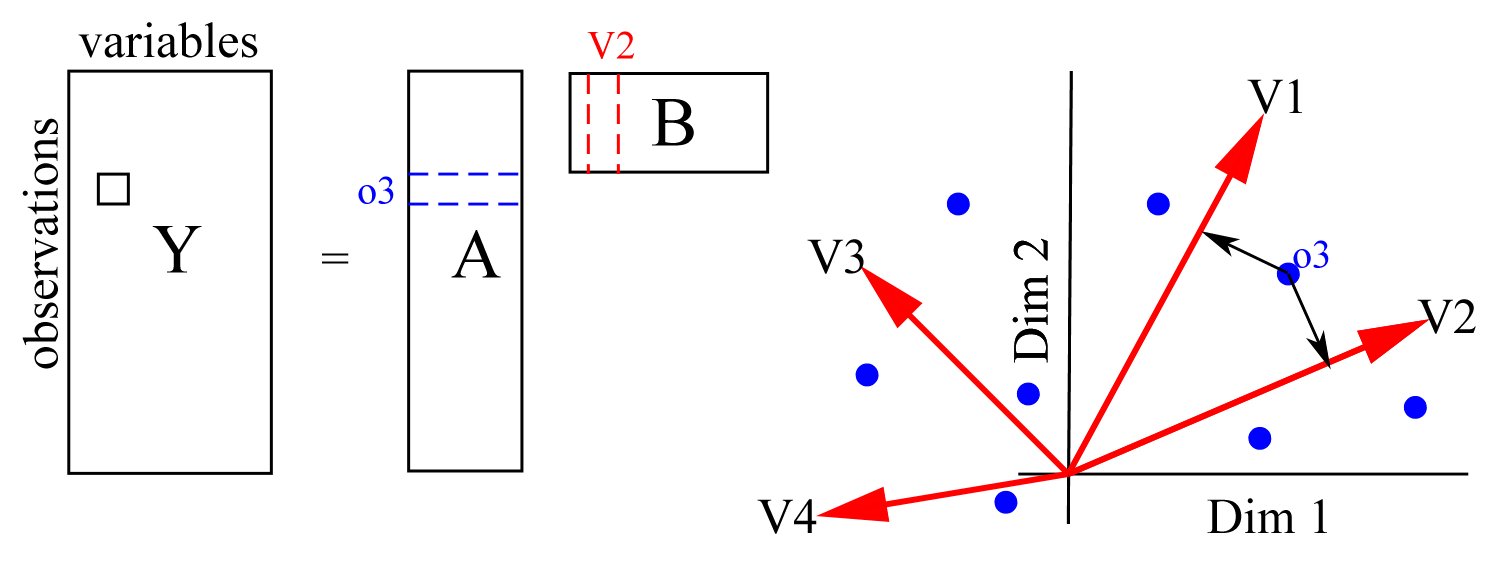
\includegraphics[width=.7\textwidth,clip]{fig/biplotdemo}
  \end{center}

%\begin{comment}
%	\item Least-squares approximation uses SVD:
%	  \begin{equation}%\label{eq:svd1}
%	  \mat{Y}^{\star}  =  \mat{U} \mat{\Lambda} \mat{V}\trans = \sum_{k=1}^{K} \lambda_k \vec{u}_k \vec{v}_k\trans
%	  \end{equation}
%
%	\item Symmetric (PCA) factorization:
%	  \begin{eqnarray*}
%	  \mat{A} & = & \mat{U} \mat{\Lambda}^{1/2} (\textrm{observation points})\\
%	  \mat{B}\trans & = & \mat{\Lambda}^{1/2} \mat{V}\trans (\textrm{variable vectors})
%	  \end{eqnarray*}
%\end{comment}
	\item Biplot properties:
  	\begin{itemize*}
	\item Plot observations as points, variables as vectors from origin (mean)
	\item Angles between vectors show correlations ($r \approx \cos (\theta)$)
	\item $y_{ij} \approx \vec{a}_i \trans \vec{b}_j$: projection of observation on variable vector
	\item Observations are uncorrelated overall (but not necessarily within group)
	\item Data ellipses for scores show low-D between and within variation
  	\end{itemize*}

  \end{itemize*}
\end{frame}

\begin{frame}
\begin{center}
  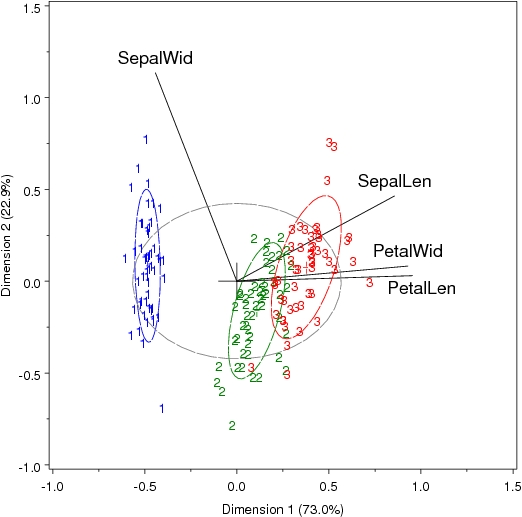
\includegraphics[height=.9\textheight,clip]{fig/bipliris}
  \\ Biplot of Iris data: \blue{\emph{setosa}: blue (1)}; \green{\emph{versicolor}: green (2)};
\red{\emph{virginca}: red (3)}
\end{center}

\end{frame}
